\documentclass[]{bytedance_seed}

% single-column: \documentclass[]{bytedance_seed}, 
%Please prioritize using single-column。

% twocolumn: \documentclass[twocolumn]{bytedance_seed}

\usepackage[toc,page,header]{appendix}


%%%%%%%%%%%%%%%%%%%%%%%%%%%%%%%%%%%%

\usepackage{minitoc}
\usepackage{cleveref} 
\usepackage{subcaption}
\usepackage{booktabs}

\usepackage{natbib}
% Standard package includes
% \usepackage{times}
\usepackage{latexsym}

% For proper rendering and hyphenation of words containing Latin characters (including in bib files)
% \usepackage[T1]{fontenc}
% For Vietnamese characters
% \usepackage[T5]{fontenc}
% See https://www.latex-project.org/help/documentation/encguide.pdf for other character sets
\usepackage{url}
\usepackage{amssymb}
\usepackage[utf8]{inputenc}
\usepackage{microtype}
\usepackage{booktabs}
\usepackage{pifont} 
\usepackage{multirow}
\usepackage{makecell}
\usepackage{paralist}
\usepackage{xspace}
\usepackage{color}
\usepackage{xcolor}
\usepackage{colortbl}
\usepackage{adjustbox}
\usepackage{hyperref} 
\usepackage[edges]{forest}
\usepackage{tikz} 
% \usepackage{longtable} % For tables that can span multiple pages
\usepackage{caption}
\usepackage{amsfonts}

\hypersetup{
    colorlinks,
    linkcolor={blue!80!black},
    citecolor={blue!80!black},
    % urlcolor={brown!50!black}
}
\tikzset{
    root/.style =             {align=center, text width=1cm, rounded corners=3pt, line width=0.3mm, fill=gray!10, draw=gray!80, font=\small},
    % demographic 
    demographic/.style =         {align=center, text width=1.8cm, rounded corners=3pt, line width=0.3mm, fill=blue!10, draw=blue!80, font=\footnotesize},
    demographic_work/.style =    {align=center, text width=10cm, rounded corners=3pt, line width=0.3mm, fill=blue!10, draw=blue!0, font=\footnotesize},
    % character 
    character/.style =         {align=center, text width=1.8cm, rounded corners=3pt, line width=0.3mm, fill=red!10, draw=red!80, font=\footnotesize},
    character_work/.style =    {align=center, text width=10cm, rounded corners=3pt, line width=0.3mm, fill=red!10, draw=red!0, font=\footnotesize},
    % Personalization
    personalization/.style =           {align=center, text width=1.8cm, rounded corners=3pt, line width=0.3mm, fill=cyan!10, draw=cyan!80, font=\footnotesize},
    personalization_work/.style =      {align=center, text width=10cm, rounded corners=3pt, line width=0.3mm, fill=cyan!10, draw=cyan!0, font=\footnotesize},
    % risks
    risk/.style =         {align=center, text width=1.8cm, rounded corners=3pt, line width=0.3mm, fill=orange!10, draw=orange!80, font=\footnotesize},
    risk_work/.style =    {align=center, text width=10cm, rounded corners=3pt, line width=0.3mm, fill=orange!10, draw=orange!0, font=\footnotesize},
}

% If the title and author information does not fit in the area allocated, uncomment the following
%
% \setlength\titlebox{7cm}
%
% and set <dim> to something 5cm or larger.
\newcommand{\new}[1]{\textcolor{purple}{{#1}}}
\newcommand{\todo}[1]{\textcolor{red}{{[$\blacksquare$ TODO: #1]}}}
\newcommand{\method}{\textsc{\textbf{DAPO}}\xspace}
\newcommand{\ie}{\textit{i.e.}\xspace}
\newcommand{\eg}{\textit{e.g.}\xspace}
\newcommand{\wo}{\textit{w/o}\xspace}
\newcommand{\dq}[1]{``#1''}
\newcommand{\sq}[1]{`#1'}
\newcommand{\cjj}[1]{\textcolor{red}{{[cjj: #1]}}}
\newcommand{\jj}[1]{\textcolor{cyan}{\small{\bf [JJ: #1]}}}
\newcommand{\qiying}[1]{\textcolor{purple}{{[qiying: #1]}}}
\newcommand{\hao}[1]{\textcolor{blue}{{[hao: #1]}}}
\newcommand{\zheng}[1]{\textcolor{brown}{{[zheng: #1]}}}
\newcommand{\hongli}[1]{\textcolor{teal}{{[hongli: #1]}}}
\newcommand{\weinan}[1]{\textcolor{orange}{{[weinan: #1]}}}


\newcommand{\etc}{\textit{etc}\xspace}
\newcommand{\cmark}{\ding{51}}
\newcommand{\xmark}{\ding{55}}
\newcommand{\customcite}[2]{\hyperlink{cite.#2}{#1}}

% \setlength\tabcolsep{3.5pt}

\newcommand\footnoteplain[1]{%
  \begingroup
  \renewcommand\thefootnote{}\footnote{#1}%
  \addtocounter{footnote}{-1}%
  \endgroup
}

\usepackage{CJK}
% \pagestyle{plain} % very strange, fixes page number centering problem.


%%%%%%%%%%%%%%%%%%%%

\title{DAPO: An Open-Source LLM Reinforcement Learning System at Scale}
% Democratizing LLM Reasoning \\ by Unveiling the Secrets of RL Scaling}
% Open-Source LLM RL System Surpassing DeepSeek's RL}
% Democratizing LLM Reasoning \\ by Unveiling the Secrets of RL Scaling}

% 

% \author[1,2,*, \dagger]{Author1}
% \author[1]{Author2}
% \author[1,2,*]{Author3}
% \author[1]{Author4}
% \author[1, \dagger]{Author5}

%论文单位请使用ByteDance Seed

\affiliation[1]{ByteDance Seed\quad $^2$Institute for AI Industry Research (AIR), Tsinghua University}
% \affiliation[2]{}
\affiliation[3]{The University of Hong Kong}
\affiliation[4]{SIA-Lab of Tsinghua AIR and ByteDance Seed}



\contribution{Full author list in Contributions}
% \contribution[*]{Work done at ByteDance Seed}
% \contribution[\dagger]{Corresponding authors}

\abstract{

%Recent research has discovered that fine-tuned 
\begin{abstract}
    
Language models are prone to dataset biases, known as shortcuts and spurious correlations in data, which often result in performance drop on new data. We present a new debiasing framework called ``\OursName'' that mitigates dataset biases by learning to be {\em undecided} in its predictions for data samples or representations associated with known or unknown biases. The framework introduces two key components: a suite of data and model perturbation operations that generate different biased views of input samples, and a contrastive objective that learns debiased and robust representations from the resulting biased views of samples. Experiments show that \OursName outperforms existing debiasing methods, particularly against out-of-domain and hard test samples without compromising the in-domain performance\footnote{Our code is available at \url{https://github.com/CLU-UML/FairFlow}.}.
\end{abstract}

% Existing debiasing methods mainly focus on detecting and re-weighting potentially biased samples in datasets. However, they have limited coverage of different types of biases and less regularization strength. 
% \OursName encodes less biases in its learned representations compared to strong baselines. 
% We illustrate that existing baselines are still biased and can be further debiased with our framework.
% , by modeling more sources of biases. 
%xx, xx .  % By explicitly modeling known biases, the proposed framework enhances the effectiveness of existing debiasing approaches. 
% We discuss how several existing approaches can be considered as special cases of \OursName.

}

% March 17, 2025
% \today

\date{March 17, 2025}
\correspondence{Qiying Yu at \email{yuqy22@mails.tsinghua.edu.cn}}

% You can add additional info fields as follows 
\checkdata[Project Page]{\url{https://dapo-sia.github.io/}}

\begin{document}

\maketitle

%不需要目录就注释掉 注意目录不要和第一页放在一块 要有\newpage
%\newpage
%\tableofcontents
%\newpage

\section{Introduction}

 % have been successful across a wide range of NLP tasks. %, paraphrase identification, sentiment analysis and relation extraction.  However, 
Existing computational models developed for natural language processing (NLP) tasks are vulnerable to dataset biases and spurious correlations in data, often referred to as ``shortcuts.''  % or annotation artifacts. 
These shortcuts enable models to achieve high performance on NLP datasets by exploiting surface-level correlations between features and labels. However, they also result in a significant performance drop on hard or slightly modified test data~\citep{naik-etal-2018-stress}. For example, in the area of natural language inference (NLI), models like BERT~\citep{devlin-etal-2019-bert} tend to misclassify premise-hypothesis pairs that contain ``negation'' words in their hypotheses as ``contradiction,'' which happen to be predictive features associated with the \textit{contradiction} label in certain NLI datasets~\citep{gururangan-etal-2018-annotation,poliak-etal-2018-hypothesis,modarressi-etal-2023-guide}.

% \hadi{related work, what has been done and what are the known findings. What's missing. cite all key papers.}

\begin{figure}[t]
    \centering
    \vspace{-20pt}
    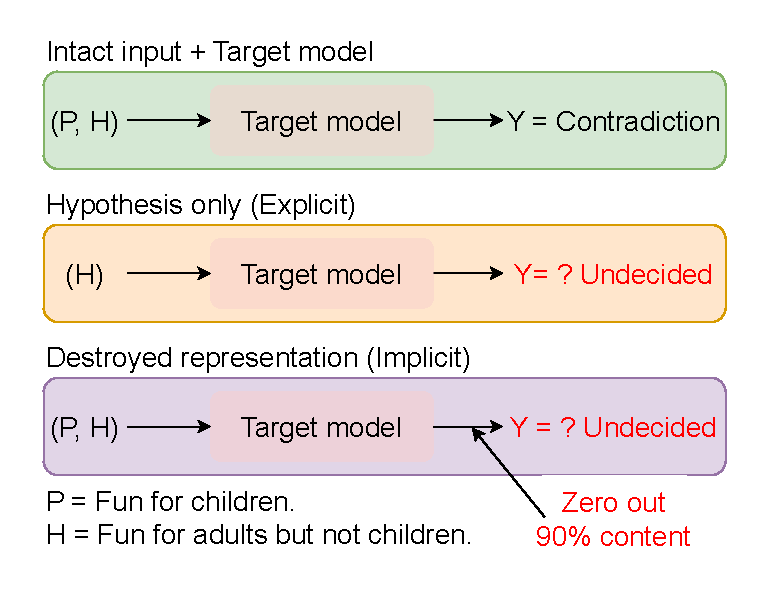
\includegraphics[width=.45\textwidth]{figure/motivating_example.pdf}
    % \vspace{-10pt}
    \caption{An example highlighting the concept of ``undecided learning'' using two types of data perturbation techniques. Given a premise-hypothesis pair in NLI, the model is expected to correctly classify their entailment relationship. However, given only the 
    % a grammatically perturbed 
    hypothesis, a robust model should be undecided, i.e., refrain from making a definite judgment 
    about the relationship between an unknown premise and %perturbed 
    the given hypothesis. Similarly, given a severely corrupted representation, a robust model should be undecided about the relation between a corrupted premise and hypothesis pair.
    Models that retain confidence in assigning labels to such inputs are likely to rely on shortcuts. \OursName takes an undecided stance against such inputs.}
    \label{fig:motivating_example}
    \vspace{-10pt}
    \label{fig:example}
\end{figure}

Existing debiasing approaches %employ external models to 
can detect known~\citep{clark-etal-2019-dont,sanh2020learning,karimi-mahabadi-etal-2020-end,modarressi-etal-2023-guide} and previously unidentified or unknown~\citep{utama-etal-2020-towards,sanh2020learning} biases in training data.
They mitigate dataset biases by 
re-weighting examples~\citep{sanh2020learning,karimi-mahabadi-etal-2020-end}, 
learning robust representations~\citep{gao-etal-2022-kernel,du-etal-2023-towards}, 
learning robust feature interaction patterns~\citep{wang-etal-2023-robust}, or 
reducing the effect of biased model components~\citep{meissner-etal-2022-debiasing}.

% Comments
% Existing
% (the original model)
% (external representations) 
% (parts)
% Any other approaches?

% \hadi{the need to investigate the missing parts. and how you do that.}s
% There are several key challenges that may compromise the effectiveness of existing approaches in mitigating dataset biases. 
Despite the significant progress made in addressing dataset biases, existing models have certain limitations:
\textbf{(a)}: they often adopt a {\em single view} to dataset biases and primarily focus on specific types of biases~\citep{clark-etal-2019-dont,karimi-mahabadi-etal-2020-end}. However, rich sources and diverse types of dataset biases can be present in the data.
\textbf{(b)}: existing approaches that are based on weak learners~\citep{utama-etal-2020-towards,sanh2020learning,ghaddar-etal-2021-end,meissner-etal-2022-debiasing} rely on a {\em single} weak learner to identify biases, which inevitably tie their performance to the capabilities of the chosen weak learner.
\textbf{(c)}: prior works often evaluate debiasing methods using BERT-based models, which may limit their generalizability to other model architectures. 

% which largely bounds these approaches by the learning capability of the weak learner.
% to insufficient regularization of model parameters against biased examples or cascade biases throughout the multi-stage training process. 
%debiasing
% Finally, existing methods are often tailored to specific NLP tasks due to the reliance on task-specific model architectures, which can restrict the transferability of the methods to different domains or problem settings. For example, Debias Mask~\citep{} does not work for embedding models, such as TransE~\citep{}. 
% We want to attend to bias when needed. 

% \hadi{2--3 key,contributions.}
We tackle the above challenges by developing \OursName--a multiview contrastive learning framework that mitigates dataset biases by being {\em undecided} in its prediction for biased views of data samples (see \textbf{Figure~\ref{fig:example}}). Specifically, the proposed method employs several data perturbation operators to generate biased views of intact data samples and integrate them into the training data and learning process. 
When presented with biased inputs, the model is trained to be undecided about the possible labels by making a uniform prediction across the label set. At the same time, the model is encouraged to be confident about intact inputs, which {\em often} serve as a reference for unbiased samples. Therefore, the approach encourages learning representations that are more attentive to the true signal of the underlying tasks rather than relying on shortcuts that are specific to certain datasets. 
In addition, the inherent randomness of the implicit perturbations in FairFlow (\S\ref{sec:imp_bias}) exposes the model to a diverse range of perturbations and prevents it from overfitting to specific types of biases present in the data.\looseness-1

The contributions of this paper are: 
\begin{itemize}
    \itemsep-1pt 
    % \itemindent-10
    \item categorization of dataset biases: we categorize prevalent data biases in NLU and model them using data perturbation operations;
    
    \item bias mitigation as an ``undecided learning'' problem: we formulate the bias mitigation problem as an ``undecided learning'' problem, which encourages reliance on genuine and task-related signals for effective debiasing;  
    % the approach can be applied to existing debiasing strategies in prior research. 
    %Specifically, in the presence of biased inputs, our approach ensures that the model's predictions are uniform across the label set, while it remains confident in predicting the labels of intact--mainly unbiased--data samples.
    \item robust performance on challengng samples: our approach shows robust results on {\em harder} test data while maintaining strong in-domain performance across several NLU tasks.\looseness-1
    % \item Our framework employs the Attention mechanism and can learn when to attend to bias and when not to. It also serves as an interpretability tool to recognize and classify spurious data.
    % \item Our framework is flexible to work with many debiasing strategies, including Product of Experts (PoE), Focal Loss (FL), etc.
    % \item We conduct extensive experiments on various types of NLP tasks, uncovering the disadvantages existing debias methods.
\end{itemize}

The experimental results show that \OursName obtains substantial improvement over competing models. Specifically, it achieves an average performance gain of 10.2 points on stress test datasets across several NLU tasks while maintaining performance on the original test sets. In addition, models trained using our framework show strong transferability, resulting in an average gain of 3.7 points in transfer testing experiments across different datasets and domains. 
Furthermore, 
% Our findings shed light on the biases present in existing debiasing methods, which still leave room for enhancement. Specifically, 
we show that existing methods can be further improved by incorporating the proposed perturbation operators within their original objectives, resulting in a substantial average improvement of 5.8 points on stress test sets across datasets. 
% with Product of Experts~\citep{10.1162/089976602760128018}. 
% In addition, we illustrate that existing debiasing methods still rely on shortcuts.



\section{Preliminary}

\subsection{Proximal Policy Optimization (PPO)}
PPO~\cite{schulman2017proximal} introduces a clipped surrogate objective for policy optimization. By constraining the policy updates within a proximal region of the previous policy using clip, PPO stabilizes training and improves sample efficiency. Specifically, PPO updates the policy by maximizing the following objective:
\begin{equation}
\begin{aligned}
\mathcal{J}_\text{PPO}(\theta) = \mathbb{E}_{(q,a)\sim \mathcal{D},o_{\le t}\sim\pi_{\theta_{\text{old}}}(\cdot\mid q)}
\Bigg[ 
\min \Bigg( \frac{\pi_{\theta}(o_t\mid q,o_{<t})}{\pi_{\theta_{\text{old}}}(o_t\mid q,o_{<t})} \hat{A}_t,  
\ \text{clip} \Bigg( \frac{\pi_{\theta}(o_t\mid q,o_{<t})}{\pi_{\theta_{\text{old}}}(o_t\mid q,o_{<t})}, 1 - \varepsilon, 1 + \varepsilon \Bigg) \hat{A}_t \Bigg) \Bigg],
\label{eq:ppoloss}
\end{aligned}
\end{equation}
where $(q,a)$ is a question-answer pair from the data distribution $\mathcal{D}$, $\varepsilon$ is the clipping range of importance sampling ratio, and $\hat{A}_t$ is an estimator of the advantage at time step $t$. Given the value function $V$ and the reward function $R$, $\hat{A}_t$ is computed using the Generalized Advantage Estimation (GAE)~\cite{schulman2018highdimensionalcontinuouscontrolusing}:
\begin{equation}
\begin{aligned}
    &\hat{A}_t^{\text{GAE}(\gamma,\lambda)} = \sum_{l=0}^{\infty}(\gamma\lambda)^l\delta_{t+l},
\end{aligned}
\end{equation}
where
\begin{equation}
    \delta_{l}=R_l+\gamma V(s_{l+1})-V(s_l),\quad 0\le\gamma,\lambda\le1.
\end{equation}


\subsection{Group Relative Policy Optimization (GRPO)}

Compared to PPO, GRPO eliminates the value function and estimates the advantage in a group-relative manner. For a specific question-answer pair $(q,a)$, the behavior policy $\pi_{\theta_\text{old}}$ samples a group of $G$ individual responses $\{ o_i\}_{i=1}^G$. Then, the advantage of the $i$-th response is calculated by normalizing the group-level rewards $\{ R_i \}_{i=1}^G$:
\begin{equation}
\hat{A}_{i,t} = \frac{r_i - \text{mean}(\{R_i\}_{i=1}^G)}{\text{std}(\{R_i\}_{i=1}^G)}.
\end{equation}

Similar to PPO, GRPO adopts a clipped objective, together with a directly imposed KL penalty term:
% Additionally, the KL-regularization between current policy $\pi_\theta$ and the reference policy $\pi_\text{ref}$ is directly added to the loss function:
\begin{equation}
\begin{aligned}
\mathcal{J}_\text{GRPO}(\theta)& = \mathbb{E}_{(q,a)\sim \mathcal{D}, \{o_i\}_{i=1}^G\sim \pi_{\theta_\text{old}}(\cdot\mid q)} \\&
\Bigg[ \frac{1}{G}\sum_{i=1}^{G} \frac{1}{|o_i|}\sum_{t=1}^{|o_i|} \Bigg( 
\min \Big( r_{i,t}(\theta) \hat{A}_{i,t},  
\ \text{clip} \Big( r_{i,t}(\theta), 1 - \varepsilon, 1 + \varepsilon \Big) \hat{A}_{i,t} \Big)
- \beta D_{\text{KL}}(\pi_{\theta} || \pi_{\text{ref}}) 
\Bigg) \Bigg],
\label{eq:grpoloss}
\end{aligned}
\end{equation}
where
\begin{equation}
    r_{i,t}(\theta)=\frac{\pi_{\theta}(o_{i,t} \mid q, o_{i,<t})}{\pi_{\theta_{\text{old}}}(o_{i,t} \mid q,o_{i,<t})}.
\end{equation}

It is also worth noting that GRPO computes the objective at the sample-level. To be exact, GRPO first calculates the mean loss within each generated sequence, before averaging the loss of different samples. As we will be discussing in Section~\ref{sec:tokenlevel}, such difference may have an impact on the performance of the algorithm.


\begin{figure}[t]
    \centering
    \begin{subfigure}{0.49\textwidth}
        \centering
        \includegraphics[width=\textwidth]{figures/3.1.2.pdf}
        \caption{Accuracies on AIME.}
        \label{fig:clighigh_acc}
    \end{subfigure}
    \hfill
    \begin{subfigure}{0.49\textwidth}
        \centering
        \includegraphics[width=\textwidth]{figures/3.1.1.pdf}
        \caption{Entropy of actor model.}
        \label{fig:cliphigh_entropy}
    \end{subfigure}
    \caption{The accuracy on the AIME test set and the entropy of the actor model's generated probabilities during the RL training process, both before and after applying \textbf{Clip-Higher} strategy.}
    \label{fig:clip_high}
\end{figure}


\subsection{Removing KL Divergence}
\label{sec:removekl}
The KL penalty term is used to regulate the
divergence between the online policy and the frozen reference policy. 
In the RLHF scenario~\cite{NEURIPS2022_b1efde53}, the goal of RL is to align the model behavior without diverging too far from the initial model.
However, during training the long-CoT reasoning model, the model distribution can diverge significantly from the initial model, thus this restriction is not necessary. Therefore, we will exclude the KL term from our proposed algorithm.

\subsection{Rule-based Reward Modeling}
The use of reward model usually suffers from the reward hacking problem~\cite{amodei2016concreteproblemsaisafety,
everitt2017reinforcementlearningcorruptedreward,
google2020specialgaming,
everitt2021rewardtamperingproblemssolutions,
gao2022scalinglawsrewardmodel,weng2024rewardhack}.
Instead, we directly use the final accuracy of a verifiable task as the outcome reward, computed using the following rule:
\begin{equation}
    R(\hat{y}, y) = 
    \begin{cases} 
    1, & \texttt{is\_equivalent}(\hat{y}, y) \\
    -1, & \text{otherwise} 
    \end{cases}
\end{equation}
where $y$ is the ground-truth answer and $\hat{y}$ is the predicted answer.
This is proved to be an effective approach to activating the base model's reasoning capability, as shown in multiple domains such as automated theorem proving~\cite{polu2020generativelanguagemodelingautomated,trinh2024solving,google2024alphageometry,google2024alphaproofandalphageometry}, computer programming~\cite{le2022coderl,shinn2023reflexionlanguageagentsverbal,chen2023teachinglargelanguagemodels,gehring2025rlefgroundingcodellms}, and mathematics competition~\cite{guo2025deepseek}.


\begin{figure*}[t]
    \centering
    \vspace{-20pt}
    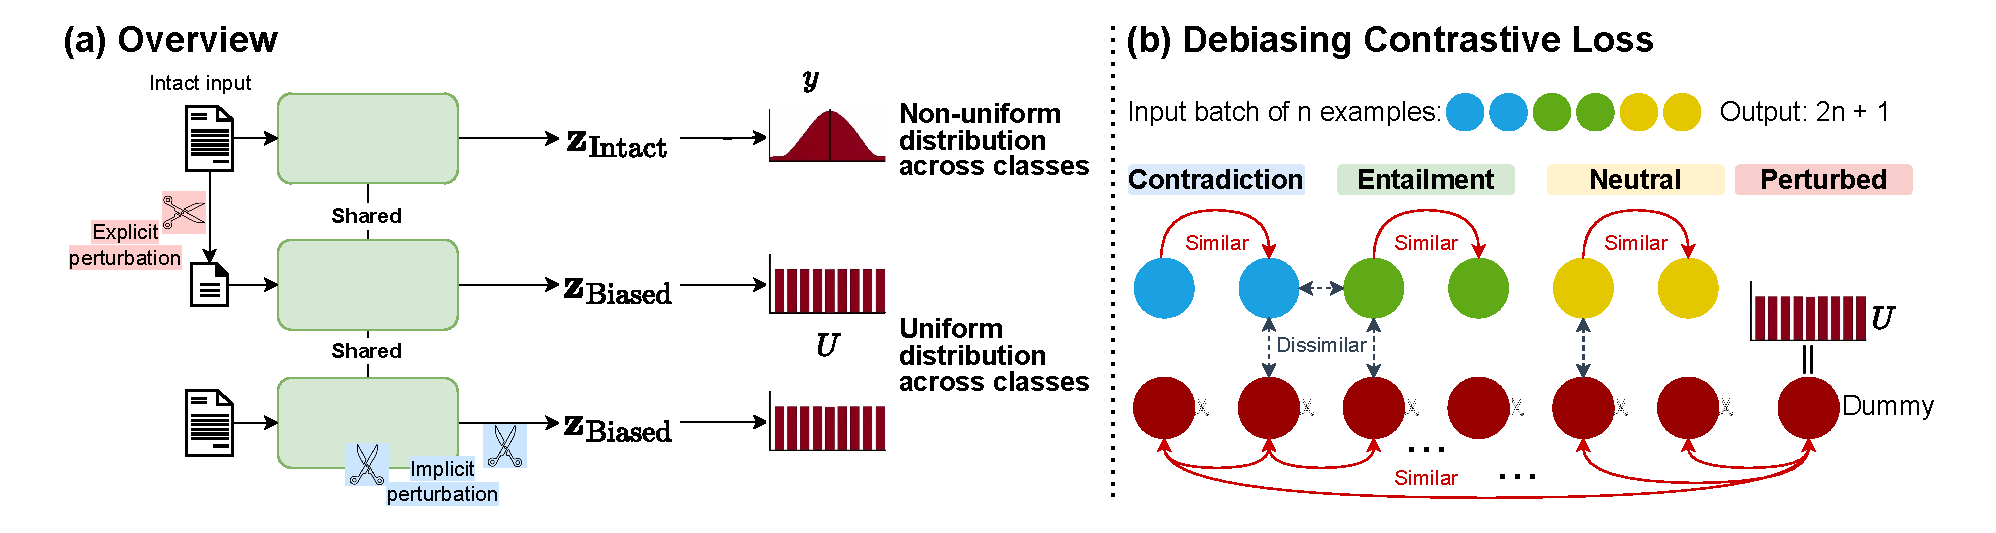
\includegraphics[width=.9\textwidth]{figure/fairflow.pdf}
    % \vspace{-20pt}
    \caption{Architecture of the proposed model. (a) Explicit and implicit perturbations are applied to inputs to obtain biased prediction $z_{\mathrm{Biased}}$. (b) Biased predictions are drawn closer to uniform distribution, while predictions for intact input are pushed away from uniform distribution through contrastive learning.}
    \label{fig:model}
    % \vspace{-10pt}
\end{figure*}

\section{Method}
\subsection{Problem Formulation}
We consider a dataset $\mathcal{D} = \{(x_i, y_i)|_{i=1}^n\}$, where $x_i$ is the $i$-th input consisting of several constituents $x_i = (x_i^1, x_i^2, \dots, x_i^p), |x_i| = p > 1$, and $y_i$ is the corresponding output for $x_i$. For example, in case of NLI, $p=2$ represents premise and hypothesis in each input and $y_i$ reflects the entailment or no-entailment relationship between the input pair. Our goal is to develop a model that is robust against different types of dataset biases in $\mathcal{D}$. 
We note that the model can be applied to a more general setting where input $x_i$ does not explicitly consist of several constituents, see \S\ref{sec:explicit_bias}.

% \subsection{A Motivating Example}
% As Figure~\ref{fig:motivating_example} shows, when given an intact premise-hypothesis pair, we want to train an NLI model to be determined about the label, since the input contains full information about the relationship between the input pair. However, if the input only contains the premise, the model should not be able to infer any information about the relationship between the premise and the hypothesis, because the hypothesis is missing. Even though the premise itself is still a valid sentence, it does not allude any signal about its relationship with another absent sentence. If a model is still confident about a label given partial input, it is very like that it relies on shortcuts to make predictions. Therefore, given such \textit{significantly corrupted instances or representations}, a robust model should remain \textit{undecided about the label}, encouraging itself to focus on causal signals rather than spurious shortcuts.


\subsection{Overview}
We categorize dataset biases as \textit{explicit} and \textit{implicit} biases. Explicit biases are readily discernible and understandable by humans, such as high degree of lexical overlap between the premise and hypothesis in case of NLI. On the other hand, implicit biases are often subtle, indiscernible to humans, and more challenging  
%linguistic (lexical or syntactic) 
% characteristics are unknown
to detect. For example, any word in input has the potential to act a shortcut, resulting in spurious correlations. 
We introduce different types of explicit and implicit biases that are {\em task-independent} and generally applicable to bias mitigation across NLP datasets (\S\ref{sec:biasmodeling}). 
%
Given such categorization, we propose a debiasing framework that mitigates dataset biases by learning genuine task-related representations that are attentive to the true signal of the tasks rather than biases and shortcut solutions in datasets. 
The key novelty of our approach is in imposing a downstream model to adopt an ``undecided'' (``uncertain'') stance in its predictions when presented with biased views of inputs. The framework achieves this goal by assigning a uniform probability across the labels, see \textbf{Figure~\ref{fig:model}}. 
Specifically, the model regularizes the loss of the target task with a contrastive loss which draws biased predictions closer to a uniform distribution while pushing other predictions away from uniform distribution (\S\ref{sec:contrastive}).  
%



% \paragraph{Bias Categorization}

% \hadi{explain/justify why each type should be considered for debiasing and how it contributes to debiasing.}

% . Some are not human perceivable. We term these biases as implicit biases. In addition to the above explicit biases, there exist other types of biases that are not as explicit as lexical or subpart bias. Other types of biases may be hard to categorize. 

% \subsubsection{Explicit Biases}
% \paragraph{Sub-input bias (explicit)} 



\subsection{Bias Modeling}\label{sec:biasmodeling}
We present a series of data perturbation operations to generate biased views by corrupting intact inputs. These perturbations can be explicit or implicit. In explicit perturbation, we directly corrupt the input data, while in implicit perturbation, we corrupt the representations of the input data. These perturbation techniques impose controlled variations on the data, which enable us to conduct a thorough analysis of their effects on bias mitigation.



% We first propose a set of data perturbations that explicitly perturb the input data. Then we model the biases in these explicitly perturbed data to force our model to make uniform predictions. We consider several types of known biases: 

\subsubsection{Explicit Biases} \label{sec:explicit_bias}
% We introduce Sub-input and Ungrammatical explicit perturbations. 

% \hadi{re lexical overlap and negation perturbations: these are tasks specific.. also, our stress sets includes these.. so our eval won't be fair as we are directly optimizing on biases that we know exist in test sets. }

% we propose a set of data perturbation operations that explicitly perturb the input data. Then we model the biases in these explicitly perturbed data and force our model to make uniform predictions.
\paragraph{Ungrammatical Perturbation} Recently, \citet{sinha-etal-2021-unnatural} showed that traditional and recent neural language models can be largely invariant to random word order permutation in their inputs. 
An ungrammatical input is often not understandable by humans and can potentially lead to explicit biases when models confidently predict outcomes for such inputs. For example, a model making a confident prediction about the contradiction class for the following perturbed premise-hypothesis pair from Figure~\ref{fig:example} may attribute its confidence to the negation term in the hypothesis: (``{\tt children fun for}'', ``{\tt children fun adults but for not}''). 
% premise: (``{\tt children fun adults but for not}'', ``{\tt children only for fun}''). 
To obtain an input with grammatical biases, we design the perturbation operation $\mathcal{P}_{Gra}$ that 
% randomly shuffles 
corrupts the word order in each input $x_i$. We encode the shuffled input using the shared encoder $f$ and transform it with a branch-specific MLP as follows:
\begin{equation}
    z_{Gra} = \texttt{MLP}_{Gra} \Big( f\big(\mathcal{P}_{Gra}(x_i) \big) \Big).
\end{equation}


\paragraph{Sub-input Perturbation} 
In NLP tasks that involve multi-part inputs (such as NLI), it is crucial to use the information from all parts of the input for prediction, i.e., all constituents should collectively contribute to accurate prediction. More importantly, an incomplete input should not lead to a confident prediction, as important information may be removed. 
Therefore, an explicit bias arises when the model makes confident predictions based on incomplete input, such as predicting the \textit{entailment} relation when only the hypothesis is provided as input in case of NLI. Sub-input biases can arise from any part of the input, denoted as $\{x_i^j\}_{j=1}^p$, or from various text spans within different sub-parts.
To realize sub-input biases, we define the $\mathcal{P}_{Sub}$ operator that takes one of the constituents of $x_i$, which is hen encoded with a shared encoder $f$ and further transferred with a constituent-specific $\texttt{MLP}_{Sub}$ as follows:
\begin{equation}
\label{eq:sub_aug}
    z_{Sub} = \texttt{MLP}_{Sub}\Big( f\big (\mathcal{P}_{Sub}(x_i)\big) \Big).
\end{equation}

\noindent We note that this operator is applicable to a more general setting where input $x_i$ does not explicitly consist of several constituents, e.g., in general text classification problems. In such cases, each $x_i$ can be divided into $p>1$ text segments. However, we acknowledge that there are tasks in which one sub-input, i.e. ${x_i^j}$ for a specific $j$, is enough to make a correct prediction for the complete input ${x_i}$, and therefore remaining undecided may seem counter-intuitive. Nevertheless, by training the model to be undecided when presented with incomplete information, we minimize the risk of biased predictions based solely on partial information, which can, in turn, make the model more robust against potential biases associated with incomplete data. 


% \paragraph{Lexical Overlap Perturbation} 
% \paragraph{Irrelevant Text Perturbation} 
% Deep learning models are vulnerable to wording of their inputs~\citep{gururangan-etal-2018-annotation}. In fact, they may focus on specific keywords and ignore the semantic and syntax analysis that is often required to effectively process the text. To obtain an input with irrelevant text biases, we design the perturbation operation $\mathcal{P}_{Irr}$  that appends irrelevant text to all the constituents of $x^i$. We encode the perturbed input using the shared encoder $f$ and transform it with a branch-specific MLP as follows:
% \begin{equation}
%     z_{Irr} = \texttt{MLP}_{Irr} \Big( f\big(\mathcal{P}_{Irr}(x_i)\big) \Big).
% \end{equation}

% \paragraph{Negation perturbation} Specific input words can have superficial correlations with labels, such as negation words in hypothesis in case of NLI. Models are prone to focus only on such superficial correlations, ignoring information from other parts. For example, BERT tends to classify examples as \textit{contradictory} because of the negation words in the hypothesis, neglecting the entailing relation between the premise and the hypothesis~\citep{karimi-mahabadi-etal-2020-end}. %Unlike previous works~\citep{}, 
% To obtain an input with negation bias, we design an perturbation operation $\mathcal{P}_{Neg}(\cdot)$ that adds negation words to the input $x^i$ as an perturbation. We encode the perturbed input using the shared encoder $f$ and transform it with a branch-specific MLP following 
% \begin{equation}
%     z_{Neg} = \texttt{MLP}_{Neg} \Big(f\big(\mathcal{P}_{Neg}(x^i)\big)\Big).
% \end{equation}


\subsubsection{Implicit Biases}
\label{sec:imp_bias}
The idea of implicit perturbations is to obtain biased representations of intact data, without explicitly perturbing the input. We introduce model- and representation-based implicit perturbation.

\paragraph{Model-based Perturbation} This approach largely perturbs a given model by converting it into a much weaker model, using mechanisms such as sparsification and layer dropping~\citep{NEURIPS2021_6e8404c3}. A weaker model is believed to capture more biases than a stronger model~\citep{ghaddar-etal-2021-end,sanh2020learning,utama-etal-2020-towards}. While existing methods require training a weak learner in advance~\citep{utama-etal-2020-towards,sanh2020learning,meissner-etal-2022-debiasing}, our method obtains biased predictions through the same deep neural model ($f$) and can be trained \emph{end-to-end}. Formally, we design a model-based perturbation operator $\mathcal{P}_{Mod}$ that uses only the first $k$ layers of the shared encoder $f$, which results in a substantially weakened model with reduced representation power. This branch encodes the intact input using the perturbed model and transform it with a branch-specific MLP as follows:
\begin{equation}
    z_{Mod} = \texttt{MLP}_{Mod} \Big( \mathcal{P}_{Mod}(f)(x_i) \Big).
\end{equation}



\paragraph{Representation-based Perturbation} This perturbation encodes the intact input with the original encoder $f$ but significantly corrupts the generated representations. Given this severely damaged and much less meaningful representation, the model should not be able to predict the correct label. We design a representation-based perturbation operator $\mathcal{P}_{Rep}$ that corrupts the intact representation, $f(x_i)$, and creates a severely perturbed representation. We then transform the perturbed representation with a branch-specific MLP as follows:
\begin{equation}
\label{eq:rep_aug}
    z_{Rep} = \texttt{MLP}_{Rep} \Big( \mathcal{P}_{Rep} \big( f(x_i) \big) \Big).
\end{equation}


% either modeling the existing biases or creating additional biases. 



% \paragraph{Perturbation}
\textbf{Table~\ref{tab:aug_list}} summarizes the above perturbation operators and provides details of their implementations. 
% DropPremise, which drops the premise part of the input; 2) DropHypothesis, which drops the hypothesis part of the input; 3) HalfHalf, which randomly takes 50\% of the tokens from each sentence; 4) Shuffle, which randomly shuffles the premise and the hypothesis; 5) DropLayer, which drops all layers after the 2nd layer; and 6) DestroyRep, which zeros out 90\% of the elements in the intact representation.




\subsection{Supervised Contrastive Debiasing}\label{sec:contrastive}
Given the explicit and implicit biased views of data samples, we expect a robust debiasing model to maintain an ``undecided'' stance across labels for biased inputs while providing confident predictions for intact inputs $x_i, \forall i$. Based on this intuition, the outputs of the bias branches should approximate a {\em uniform distribution} ($U$) across classes, while the output of the original branch should align with its corresponding gold distribution, i.e., the label $y_i$. 
% Through back-propagation, we can achieve the goal of debiasing the representations of the backbone model. 
To achieve this goal, we adapt the supervised contrastive loss~\citep{khosla2020supervised}, which operates by first grouping samples based on their respective labels, and then encouraging predictions (logits) of pairs within the same group to become closer while pushing logits of pairs across different groups further apart, i.e. forming positive pairs within the same group while creating negative pairs using all other pairs: % (see footnote 2).
% i.e. forming positive pairs within the same group while creating negative pairs across different groups.

\begin{table}\small
\centering
\setlength{\tabcolsep}{3pt}
\renewcommand{\arraystretch}{1} 
\begin{tabular}{c|c|l}
\toprule
\textbf{Operator}               & \textbf{Type}     & \textbf{Implementation} \\
\midrule
$\mathcal{P}_{Gra}$ & Explicit & Shuffle tokens in $x_i$ randomly \\
$\mathcal{P}_{Sub}$  & Explicit & Drop $1/p$ of tokens from $x_i^j$ randomly \\
$\mathcal{P}_{Sub}$  & Explicit & Drop $x_i^j, j=1\dots p$ \\
% $\mathcal{P}_{Irr}$  & Explicit & Add same irrelevant text to all $x_i^j$ \\
% $\mathcal{P}_{Neg}$  & Explicit & Add negation words to all $x^i_p$ \\
\midrule
$\mathcal{P}_{Mod}$  & Implicit & Use only first $k$ of layers of $f$\\
$\mathcal{P}_{Rep}$  & Implicit & Zero out $m\%$ of values in $f(x_i)$ \\
\bottomrule
  \end{tabular}
  \caption{Implementations of proposed perturbations}
  \label{tab:aug_list}
  \vspace{-10pt}
\end{table}


We adapt this loss function for bias mitigation as follows (described for a single perturbation for simplicity):
given a batch of $n$ non-perturbed examples, we perturb them using a perturbation technique described in Table~\ref{tab:aug_list}. The perturbed examples form a single group as they all have the same label (a uniform distribution across all classes), and the non-perturbed examples with the same label form separate groups.\footnote{For example, four groups in case of NLI: perturbed examples, non-perturbed examples labeled as `entailment', non-perturbed examples labeled as `contradiction', and non-perturbed examples labeled as `neutral'.} 
As illustrated in \textbf{Figure~\ref{fig:model}}, we encourage the model to be undecided about the label of perturbed inputs by adding a dummy example that has a ``fixed'' uniform distribution across all labels to the group of perturbed examples, resulting in a batch of $2n+1$ examples ($\mathcal{I}$). We compute the contrastive loss as follows:
\begin{multline}
\label{eq:supcontras}
    \mathcal{L}_{\mathrm{Debias}} = \\ 
    \sum_{i \in \mathcal{I}} \frac{-1}{|\mathcal{G}(i)|} \sum_{j \in \mathcal{G}(i)} \mathrm{log} \frac{\mathrm{exp} (z_i \cdot z_j / \tau)}{\sum_{k \in \mathcal{A}(i)} \mathrm{exp} (z_i \cdot z_k / \tau)},
\end{multline}
where $\mathcal{G}(i)$ is the set of examples that are in the same group as $i$ (having the same label as $i$); 
$\mathcal{A}(i) = \mathcal{I}\backslash\{i\}$ is the set of all examples except $i$; 
$z$ indicates the logit of an example, which for perturbed examples is obtained from one of the Equations (\ref{eq:sub_aug})--(\ref{eq:rep_aug}); and 
$\tau$ denotes the temperature parameter.\footnote{We note that the summation over all samples except $i$ in the denominator of (\ref{eq:supcontras}) is motivated by noise contrastive estimation and N-pair losses~\citep{khosla2020supervised,pmlr-v9-gutmann10a,NIPS2016_6b180037}, in which the ability to discriminate between signal and noise (negative class) is improved by adding more examples of negative class.} The dummy example in the perturbed group has a fixed uniform distribution across all labels as its $z$. This formulation encourages the model to be undecided about the label of perturbed inputs, while being confident about the labels of intact inputs, allowing it to effectively distinguish between different groups of examples. 

% Given the logit of each example non-perturbed example $z_i$ from Equations \ref{eq:sub_aug}--\ref{eq:rep_aug}, ee enforce $z_{2N+1}$ to be a ``fixed'' uniform distribution across all labels, which can be thought of as adding a dummy example of uniform distribution to the group of perturbed examples. This dummy example is used for creating positive pairs for examples within the perturbed group. This adjustment enables the model to learn representations that can effectively distinguish between perturbed and non-perturbed examples. Given an index $i$, $G(i)$ denotes the indices in $I$ from the same group of $i$. The contrastive debiasing loss is defined as % If the $i$-th example is non-perturbed, $P(i)$ denotes the indices of the examples whose labels are the same as $i$'s. If the $i$-th example is perturbed, $P(i)$ denotes the indices of uniform distribution. We enforce the logits $z_p$ in the numerator of Eq.~\ref{eq:supcontras} 



% $A(i) = I\backslash\{i\}$ and $\tau$ denotes the temperature parameter. This formulation encourages the model to be undecided about the label of partial or significantly perturbed inputs, while being confident about the labels of intact inputs.



% a two-step process: 1) sample augmentation and 2) grouping based on class labels. To adapt it for bias mitigation, we follow the same process but adopt different augmentation and grouping methods. Specifically, given a batch of examples, we first perturb the examples with our proposed perturbations in Table~\ref{tab:aug_list}. Next, perturbed examples form a single group as they all have the same label (a uniform distribution across all labels), and non-perturbed examples with the same label form separate groups. For instance, in the context of the NLI task, this adaptation results in four distinct groups: perturbed examples, non-perturbed examples labeled as 'entailment', non-perturbed examples labeled as 'contradiction', and non-perturbed examples labeled as 'neutral'. Examples from the same group are encouraged to be similar, while examples across groups are encouraged to be dissimilar.

% Formally, we describe our proposed loss function with a single perturbation, which can be extended to multiple perturbations. Given a batch of $N$ examples, we randomly sample $p \in \mathcal{P}$ to transform the batch into a multiviewed batch, where $i \in I \buildrel\Delta\over = \{1, 2, ..., 2N+1 \}$ denotes the index of examples. We first obtain their representations $z_i \forall i \in I$, depending on what perturbation is applied to the example following Equations \ref{eq:sub_aug}--\ref{eq:rep_aug}, with $z_i = f(x_i)$ as the non-perturbation representation. We enforce $z_{2N+1}$ to be a ``fixed'' uniform distribution across all labels, which can be thought of as adding a dummy example of uniform distribution to the group of perturbed examples. This dummy example is used for creating positive pairs for examples within the perturbed group. This adjustment enables the model to learn representations that can effectively distinguish between perturbed and non-perturbed examples. Given an index $i$, $P(i)$ denotes the indices in $I$ from the same group of $i$. The contrastive debiasing loss is defined as % If the $i$-th example is non-perturbed, $P(i)$ denotes the indices of the examples whose labels are the same as $i$'s. If the $i$-th example is perturbed, $P(i)$ denotes the indices of uniform distribution. We enforce the logits $z_p$ in the numerator of Eq.~\ref{eq:supcontras} 
% \begin{multline}
% \label{eq:supcontras}
%     \mathcal{L}_{\mathrm{Debias}} = \\ 
%     \sum_{i \in I} \frac{-1}{|P(i)|} \sum_{p \in P(i)} \mathrm{log} \frac{\mathrm{exp} (z_i \cdot z_p / \tau)}{\sum_{a \in A(i)} \mathrm{exp} (z_i \cdot z_a / \tau)},
% \end{multline} where $A(i) = I\backslash\{i\}$ and $\tau$ denotes the temperature parameter. This formulation encourages the model to be undecided about the label of partial or significantly perturbed inputs, while being confident about the labels of intact inputs.


% $\mathcal{P}(i) \buildrel\Delta\over =  \{x^i_j\}_{j=1}^P$
% \begin{equation}
%     l = - log \frac{sim(i, j)}{\sum }
% \end{equation}
% \begin{equation}
%     \mathcal{L}_{Debias} = \mathcal{L}_{Intact} + \mathcal{L}_{Bias},
% \end{equation}
% \begin{equation} 
% \label{eq:intact}
%     \mathcal{L}_{Intact} = \mathbb{KL}(z_{Intact}||y) - \mathbb{KL}(z_{Intact}||U),
% \end{equation}
% \begin{equation}
% \label{eq:bias}
%     \mathcal{L}_{Bias} = \mathbb{KL}(z_{Bias}||U) - \mathbb{KL}(z_{Bias}||y),
% \end{equation}

% where $\mathbb{KL}(q||p)$ denotes the KL-Divergence and $U$ denotes the uniform distribution over the labels. 
% Equation \ref{eq:intact} encourages the model to be confident about the labels of intact inputs, while Equation \ref{eq:bias} encourages our model to be undecided about the labels of biased inputs.
%
Finally the model learns the debiasing task in an \emph{end-to-end} manner by minimizing the standard cross-entropy loss with predictions of intact input $z_{\mathrm{Intact}}=f(x_i)$ and the debiasing loss, weighted by a balancing hyperparameter $\lambda$ as follows:
\begin{equation}
    \theta^{*} = \arg\min_{\theta} \mathcal{L}_{\mathrm{CE}}(z_{\mathrm{Intact}}, y_i) + \lambda \mathcal{L}_{\mathrm{Debias}}.
\end{equation}




% \begin{table}\small
% \centering
% \setlength{\tabcolsep}{3.9pt}
% \renewcommand{\arraystretch}{0.9} 
% \begin{tabular}{c|c|l}
% \toprule
% Method               & Type     & Implementation \\
% \midrule
% $\mathcal{P}_{Sub}$  & Explicit & Drop $x_i^p$ \\
% $\mathcal{P}_{Sub}$  & Explicit & Drop $1/p$ of tokens from each $x^i_p$ randomly \\
% $\mathcal{P}_{Gra}$ & Explicit & Shuffle tokens in $x^i$ randomly \\
% $\mathcal{P}_{Irr}$  & Explicit & Add same irrelevant text to all $x^i_p$ \\
% % $\mathcal{P}_{Neg}$  & Explicit & Add negation words to all $x^i_p$ \\
% \midrule
% $\mathcal{P}_{Mod}$  & Implicit & Use only first 20\% of layers of $f$\\
% $\mathcal{P}_{Rep}$  & Implicit & Zero out 90\% of $f(x^i)$ \\
% \bottomrule
%   \end{tabular}
%   \caption{Implementations of proposed perturbations}
%   \label{tab:aug_list}
%   \vspace{-10pt}
% \end{table}
% Sup contras loss
% We adopt the Supervised Contrastive Learning loss~\citep{khosla2020supervised} shown in (\ref{eq:supcontras}) to achieve our contrastive learning objective:
% \begin{multline}
% \label{eq:supcontras}
%     \mathcal{L}^{sup}(z_i) = \sum_{i \in I} \mathcal{L}^{sup}_{out, i} = \\ 
%     \sum_{i \in I} \frac{-1}{|P(i)|} \sum_{p \in P(i)} \mathrm{log} \frac{\mathrm{exp} (z_i \cdot z_p / \tau)}{\sum_{a \in A(i)} \mathrm{exp} (z_i \cdot z_a / \tau)},
% \end{multline} where $A(i) \buildrel\Delta\over =  \{x^i_j\}_{j=1}^P$ denotes a multiviewed batch of the $i$-th example, $P(i)$ denotes the indices of examples in $A(i)$ whose label is the same as $i$'s, $z_i$ denotes the representation of the $i$-th example, and $\tau$ denotes the temperature parameter that is used for smoothness and hard negatives purposes~\citep{khosla2020supervised}. %...

% Given an input example $(x, y)$ with $P$ constituents in $x$, we first obtain the outputs from all the branches as described in \S\ref{sec:bias_branch}. We then apply the contrastive objective to learn debiased representations. For the output of the original branch $z_O$, we consider the uniform distribution $U$ as the negative example and the biased distribution $y$ as the positive example. For the output of any bias branch $z_B$, we consider $U$ as the positive example and $y$ as the negative example. 

% Finally, we combine the original Cross-Entropy Loss and the contrastive loss, weighted by a balancing factor $\lambda$. The final loss is defined as 
% \begin{multline}
%     \mathcal{L} = \mathcal{L}_{\mathrm{CE}}(z_O, y) + \lambda (\mathcal{L}^{sup}(z_O) + \\ \mathcal{L}^{sup}(z_L) + \mathcal{L}^{sup}(z_W) + \sum_{p} \mathcal{L}^{sup}(z_p)).
% \end{multline}


\paragraph{Compatibility and Difference with Other Debiasing Objectives and Training Methods} Our framework is designed to be %provide flexibility and adaptability 
compatible with debiasing objectives in existing literature. Notably, it can incorporate objectives such as the product of experts (PoE)~\citep{karimi-mahabadi-etal-2020-end,clark-etal-2019-dont}, debiased focal loss~\citep{karimi-mahabadi-etal-2020-end}, and other possible objectives, see Appendix~\ref{sec:debias_obj} for more details. In experiments, we show that our framework can further improve these well-performing baseline models. One major difference with existing debiasing objectives is that prior works use a biased model to measure how much biases present in input, while \OursCL encourages robust models to be undecided given known biased inputs, obtained by the proposed perturbations.
Moreover, we do not impose any restriction on the parametrization of the underlying model $f$, making our framework flexible to work with a wide range of training methods and network architectures (Table~\ref{tab:roberta}-\ref{tab:gpt2} in Appendix).


\section{Experiments}

% \subsection{Setup}
\paragraph{Setup}
We employ BERT~\citep{devlin-etal-2019-bert} as the commonly-used base model in previous works. In addition, we extend our evaluation to RoBERTa~\citep{liu2019roberta} and GPT-2~\citep{radford2019language} for a more comprehensive analysis.

\paragraph{Datasets} We evaluate our debiasing framework on three NLP datasets including 
MNLI~\citep{williams-etal-2018-broad}, 
paraphrase identification using Quora question pairs (QQP)~\citep{sharma2019natural}, and
relation extraction using gene-phenotype relation (PGR)~\citep{sousa-etal-2019-silver}. 
% We use their corresponding \textbf{In-Domain Test Sets} for evaluation.
These datasets are used for {\em in-domain} (ID) evaluation.

\paragraph{Stress Test Sets} We assess the robustness of models against spurious correlations using ``stress test sets,'' specifically designed with hard examples to challenge models. 
% We test if models are robust to spurious correlations with \textit{stress test sets} which contain hard examples created to fool models. 
We use the stress test set for MNLI from~\citep{naik-etal-2018-stress}, and
use the same approach to generate the stress test set for QQP.
% following the same label preserving rules from~\citep{naik-etal-2018-stress}. 
For PGR, the label-preserving rules from previous tasks do not apply due to the nature of this dataset.
% the above rules are not be applicable since it doesn't align with the nature of the task. However, 
However, given the long-tail distribution of entity appearances, we create a stress test set for PGR by selecting test examples in which both entities appear less than five times in the training set.

\paragraph{OOD Test Sets} We assess the performance of models on existing out-of-distribution (OOD) test sets, which serve as another challenge benchmark. For MNLI, we use HANS~\citep{mccoy-etal-2019-right}, which is designed to test models' capabilities against lexical and syntactic heuristics in data. For QQP, we employ the PAWS dataset~\citep{zhang-etal-2019-paws}, which focuses on paraphrase identification in cases of high lexical and surface-level similarity between question pairs.

\paragraph{Transfer Test Sets} We evaluate the performance of models in maintaining strong transferability across datasets. We use SNLI~\citep{bowman-etal-2015-large} and MRPC~\citep{dolan-brockett-2005-automatically} as the transfer set for MNLI and QQP, respectively. 
% \paragraph{Probing set}
% Previous work~\citep{mendelson-belinkov-2021-debiasing} discovered that debiased models can be still biased. We use the probing set to probe if there still exists dataset bias in our model.

\begin{table*}
\tiny
\centering
% \setlength{\tabcolsep}{3.9pt}
% \renewcommand{\arraystretch}{0.9} 
\begin{tabular}{l|cccc|cccc|cc|cccc}
\toprule
\multirow{2}{2em}{\textbf{Model}} & \multicolumn{4}{c|}{\textbf{MNLI} (Acc.)} & \multicolumn{4}{c|}{\textbf{QQP} (F1)} & \multicolumn{2}{c|}{\textbf{PGR} (F1)} & \multicolumn{4}{c}{\textbf{Avg.}}\\
               & ID   & Stress & OOD & Transfer & ID & Stress & OOD & Transfer & ID & Stress & ID & Stress & OOD & Transfer \\ 
    \toprule
    \textbf{\FT}        & 84.3 & 61.7 & 59.7 & 78.7 & 88.6 & 63.3 & 47.7 & 65.1 & 64.3 & 55.2 & 79.1 & 60.1 & 53.7 & 71.9 \\ 
    \midrule
    \textbf{\MASK}      & 83.5 & 59.7 & 59.7 & 78.3 & 88.1 & 64.6 & 50.3 & 68.5 & 64.1 & 51.7 & 78.6 & 58.7 & 55.0 & 73.4 \\ 
    \textbf{\KW}        & 84.0 & 60.9 & 60.2 & 78.4 & 88.8 & 65.1 & 51.2 & 69.6 & 64.3 & 51.8 & 79.0 & 59.3 & 55.7 & 74.0 \\ 
    \textbf{\ETE}       & 83.4 & 61.3 & 62.3 & 77.5 & 88.5 & 64.5 & 51.4 & 70.5 & 63.0 & 53.6 & 78.3 & 59.8 & 56.8 & 74.0 \\
    \textbf{LSWC}       & 80.7 & 59.4 & 59.3 & 77.7 & 87.1 & 65.8 & 49.6 & 70.0 & 63.3 & 52.8 & 77.0 & 59.3 & 54.5 & 73.8 \\ 
    \textbf{\IE}        & 84.1 & 61.8 & 62.7 & 78.1 & 87.6 & 63.5 & 53.0 & 68.3 & 64.2 & 54.9 & 78.6 & 60.1 & 57.9 & 73.2 \\
    \textbf{\READ}      & 80.8 & 61.5 & 63.4 & 75.1 & 87.0 & 66.7 & 53.6 & 68.2 & 63.0 & 54.4 & 76.9 & 60.9 & 58.5 & 71.7 \\ 
    \midrule
    \textbf{\OursPoe}   & 84.6 & 64.3 & 64.3 & 79.5 & 88.8 & 71.0 & 53.9 & 70.4 & 64.9 & 55.9 & 79.4 & 63.7 & 59.1 & \underline{75.0} \\ 
    \textbf{\OursFocal} & \underline{84.9} & \underline{64.8} & \underline{64.3} & \underline{79.3} & \underline{89.5} & \underline{71.3} & \underline{54.9} & \underline{70.7} & \underline{65.4} & \underline{56.5} & \underline{79.9} & \underline{64.2} & \underline{59.6} & \underline{75.0} \\
    \textbf{\OursCL}    & \textbf{85.1} & \textbf{65.4} & \textbf{64.9} & \textbf{79.6} & \textbf{90.4} & \textbf{72.0} & \textbf{56.0} & \textbf{72.4} & \textbf{65.9} & \textbf{56.6} & \textbf{80.5} & \textbf{64.7} & \textbf{60.5} & \textbf{76.0} \\ 
    \bottomrule
  \end{tabular}
  \caption{Experimental results on three datasets averaged across three architectures. Results for each architecture are shown in Table~\ref{tab:bert}-\ref{tab:gpt2} in Appendix. The best performance is in \textbf{bold} and the second best is \underline{underlined}.}
  \label{tab:main}
\end{table*}


\begin{table*}
\small
\centering
\begin{tabular}{l|cccc}
\toprule
\multirow{2}{*}{\textbf{Model}} & \multicolumn{4}{c}{\textbf{Avg.}}\\
                & ID & Stress & OOD & Transfer \\ 
    \midrule
    \textbf{\FT}        & 79.1 & 60.1 & 53.7 & 71.9 \\ 
    \midrule
    \textbf{\ETE}       & 78.3 & 59.8 & 56.8 & 74.0 \\
    \textbf{\MASK}      & 78.6 & 58.7 & 55.0 & 73.4 \\ 
    \textbf{LSWC}       & 77.0 & 59.3 & 54.5 & 73.8 \\ 
    \textbf{\IE}        & 78.6 & 60.1 & 57.9 & 73.2 \\
    \textbf{\KW}        & 79.0 & 59.3 & 55.7 & 74.0 \\ 
    \textbf{\READ}      & 76.9 & 60.9 & 58.5 & 71.7 \\ 
    \midrule
    \textbf{\OursPoe}   & 79.4 & 63.7 & 59.1 & \underline{75.0} \\ 
    \textbf{\OursFocal} & \underline{79.9} & \underline{64.2} & \underline{59.6} & \underline{75.0} \\
    \textbf{\OursCL}    & \textbf{80.5} & \textbf{64.7} & \textbf{60.5} & \textbf{76.0} \\ 
    \bottomrule
  \end{tabular}
\end{table*}


\paragraph{Baselines} 
We consider the following baselines:
\vspace{-5pt}
\begin{itemize}
    \itemsep-2pt
    \itemindent-10pt
    \item \textbf{\FT} standard finetuning without debiasing based on the base model used. 
    % \item \textbf{Rubi}~\citep{cadene2019rubi}, which models the bias of input texts to re-weight the prediction loss in text-image classification. In our experiments, we replace the image encoder in Rubi with a text encoder.
    \item \textbf{\ETE}~\citep{karimi-mahabadi-etal-2020-end}, which trains a biased model on the hypothesis only and trains a robust model using Product of Experts (PoE)~\citep{10.1162/089976602760128018}.
    \item \textbf{\MASK}~\citep{meissner-etal-2022-debiasing}, which first trains a weak learner and then prunes the robust model using PoE. %odel.
    \item \textbf{\KW}~\citep{gao-etal-2022-kernel}, which learns isotropic sentence embeddings using Nystr\"{o}m kernel approximation~\citep{Xu_Jin_Shen_Zhu_2015} method, achieving disentangled correlation between robust and spurious embeddings.
    \item \textbf{LWBC}~\citep{kim2022learning}, which learns a debiased model from a commitee of biased model obtained from subsets of data.
    \item \textbf{\IE}~\citep{du-etal-2023-towards}, which mitigates dataset biases with an ensemble of random biased induction forest; the model induces a set of biased features and then purifies the biased features using information entropy\footnote{While this method does not have a publicly released code, we tried our best to reproduce their approach and results with a few points lower than reported.}.
    \item \textbf{\READ}~\citep{wang-etal-2023-robust}, which assumes that spuriousness comes from the attention
    % of \texttt{[CLS]} over other tokens 
    and proposes to do deep ensemble of main and biased model at the attention level to learn robust feature interaction.
\end{itemize}




% \input{sections/050discussion}
% \section{Related Work}

\subsection{Reasoning Models}

\subsection{Reinforcement Learning}

\section{Conclusion}

In this paper, we release a fully open-sourced system for large-scale LLM RL, including algorithm, code infrastructure, and dataset. The system achieves state-of-the-art large-scale LLM RL performance (AIME 50 using Qwen-32B pretrained model). We propose the \textbf{D}ecoupled Clip and \textbf{D}ynamic s\textbf{A}mpling \textbf{P}olicy \textbf{O}ptimization (\textbf{DAPO}) algorithm, and introduce 4 key techniques to make RL powerfully effective and efficient in the long-CoT RL scenario.
Additionally, by open-sourcing the training code and dataset, we provide the broader research community and society with practical access to a scalable reinforcement learning solution, enabling all to benefit from these advancements. 

\newpage

\section*{Contributions}

\textbf{Project Lead}\quad 

Qiying Yu$^{1,2,4}$

% \subsection*{Algorithm}

\textbf{Algorithm}

Qiying Yu$^{1,2,4}$, Zheng Zhang$^{1}$, Ruofei Zhu$^{1}$, Yufeng Yuan$^{1}$, Xiaochen Zuo$^{1}$, Yu Yue$^{1}$

% \subsection*{Infrastructure$^{*}$}

\textbf{Infrastructure$^{*}$}

Tiantian Fan$^{1}$, Gaohong Liu$^{1}$, Lingjun Liu$^{1}$, Xin Liu$^{1}$, Haibin Lin$^{1}$, Zhiqi Lin$^{1}$, Bole Ma$^{1}$, Guangming Sheng$^{1,3}$, Yuxuan Tong$^{1,2,4}$, Qiying Yu$^{1,2,4}$, Chi Zhang$^{1}$, Mofan Zhang$^{1}$, Wang Zhang$^{1}$, Hang Zhu$^{1}$, Jinhua Zhu$^{1}$

$^{*}$Last-Name in Alphabetical Order

% \subsection*{Dataset}

\textbf{Dataset}

Jiaze Chen$^{1}$, Jiangjie Chen$^{1,4}$, Chengyi Wang$^{1}$, Hongli Yu$^{1,2,4}$, Weinan Dai$^{1,2,4}$, Yuxuan Song$^{1,2,4}$, Xiangpeng Wei$^{1}$, Qiying Yu$^{1,2,4}$

% \subsection*{Supervision}

\textbf{Supervision}

Hao Zhou$^{2,4}$, Jingjing Liu$^{2,4}$, Wei-Ying Ma$^{2,4}$, Ya-Qin Zhang$^{2,4}$, Lin Yan$^{1,4}$, Mu Qiao$^{1,4}$, Yonghui Wu$^{1}$, Mingxuan Wang$^{1,4}$

% \subsection*{Affiliation}

\textbf{Affiliation}

% $^1$\textsf{ByteDance Seed}

% $^2$\textsf{Institute for AI Industry Research (AIR), Tsinghua University}

% $^3$\textsf{The University of Hong Kong}

% $^4$\textsf{SIA-Lab of Tsinghua AIR and ByteDance Seed}

$^1$ByteDance Seed

$^2$Institute for AI Industry Research (AIR), Tsinghua University

$^3$The University of Hong Kong

$^4$SIA-Lab of Tsinghua AIR and ByteDance Seed

\section*{Acknowledgments}

We thank Zhengyin Du, Kai Shen, Tianyang Zhan, Zhen Xiao, Renjie Zheng, Li Han, Kaihua Jiang as well as other colleagues at ByteDance for their support for the \method project.

\clearpage

\bibliographystyle{unsrt}
% \bibliographystyle{plainnat}
\bibliography{main}

\clearpage

\beginappendix

\section{Hello World}
%\subsection{Hello World}

\end{document}